% !TEX program = pdflatex
\documentclass[11pt,a4paper]{article}

% --- packages (kept minimal and standard) ---
\usepackage[utf8]{inputenc}
\usepackage[T1]{fontenc}
\usepackage{lmodern}
\usepackage{geometry}
\geometry{margin=1in}
\usepackage{amsmath,amssymb}
\usepackage{siunitx}
\usepackage{graphicx}
\usepackage[font=small,labelfont=bf,labelsep=endash]{caption}
\usepackage{booktabs}
\usepackage{physics}
\usepackage{hyperref}
\hypersetup{colorlinks=true,linkcolor=blue,citecolor=blue,urlcolor=blue}

% --- title & author ---
\title{Design Methodology for a Dual-Jet Hovering Disc Using Concentric Air Curtains}
\author{ }
\date{ }

\begin{document}
\maketitle

\begin{abstract}
This work presents a physical model and an operational design methodology for a hovering disc sustained by two concentric air jets. The outer annular jet forms an aerodynamic curtain that confines the inner flow and minimizes leakage, whereas the inner jet compensates the residual mass loss to maintain a controlled cushion pressure beneath the disc. Unlike thin-film or incompressible assumptions, the analysis adopts a low-Mach \emph{compressible}, axisymmetric model over a finite-height domain with height comparable to radius. The paper states the governing equations for lift, leakage, and curtain dynamics, and provides an algorithm to compute pressure and velocity profiles over the entire $(r,z)$ domain to achieve stable hovering with minimal power.
\end{abstract}

\section{Introduction and Operating Principle}
The device is a rigid circular disc of total radius $R_{\text{tot}}$ hovering at a distance $h$ from the ground by sustaining an overpressure $p_c$ in the central region. Two coaxial jets are employed (Fig.~\ref{fig:geometry}): an \emph{outer annular jet} (``corona'') acting as an air curtain that seals and recirculates the cushion flow, and an \emph{inner jet} that compensates residual mass leakage across the periphery. The design goal is to select geometry and jet operating points so that the target payload $W$ is carried with acceptable power and stability margins.

\section{Assumptions and Computational Domain}
We explicitly state the assumptions used throughout the model:
\begin{itemize}
  \item \textbf{Axisymmetry.} The flow is axisymmetric with no swirl. The computational domain is the \emph{positive half-plane} $(r\ge 0,\, z\ge 0)$.
  \item \textbf{Finite-height domain, no thin-film hypothesis.} Height and radius are \emph{comparable}: $h \sim R_{\text{tot}}$; no $h\ll R$ assumption is made.
  \item \textbf{Compressible, low-Mach gas.} Air obeys the ideal-gas law $p=\rho R_g T$, with Mach numbers sufficiently low to avoid shock waves, but allowing density and temperature variations.
  \item \textbf{Domain filled only with air.} In the region $r\in[0,R_{\text{tot}}]$, $z\in[0,h]$ there are \emph{no solid obstacles}: the volume is entirely filled with air at different $(p,T,\mathbf{v})$. The \emph{boundaries} are the ground ($z=0$), the disc underside ($z=h$), the axis ($r=0$), and the outer radial boundary ($r=R_{\text{tot}}$).
  \item \textbf{Outer curtain and leakage annulus.} The air curtain is issued from a slot of thickness $b$ at $r\approx R_{\text{tot}}$ and turns near the ground to provide sealing. The leakage ring has width $w$ so that the inner “core” extends to $R^-=R_{\text{tot}}-w$.
  \item \textbf{Steady, mean flow.} The analysis targets mean fields; acoustic fluctuations are neglected.
\end{itemize}

\section{Geometry and Notation}
We adopt the following notation, consistent with the schematic in Fig.~\ref{fig:geometry}:
\begin{itemize}
  \item $R_{\text{tot}}$ total disc radius; $R^-=R_{\text{tot}}-w$ inner edge of the leakage annulus of width $w$;
  \item $h$ nominal clearance to the ground;
  \item $p_c$ target cushion overpressure (area-averaged), $W$ payload;
  \item Outer jet (\textit{corona}): mass flow $\dot m_{\mathrm{corona}}$, slot thickness $b$, slot area $A_{\mathrm{corona}}=2\pi R_{\text{tot}}\,b$, exit speed $U_{\mathrm{corona}}=\dot m_{\mathrm{corona}}/(\rho_j A_{\mathrm{corona}})$ with jet density $\rho_j$;
  \item Inner jet: mass flow $\dot m_{\mathrm{in}}$ (fills residual losses);
  \item Mass loss across the periphery: $\dot m_{\mathrm{loss}}$; volumetric loss $Q_{\mathrm{loss}}=\dot m_{\mathrm{loss}}/\rho_\mathrm{edge}$ with $\rho_\mathrm{edge}=\rho\!\big(p_\mathrm{edge},T_\mathrm{edge}\big)$.
\end{itemize}

\begin{figure}[t]
  \centering
  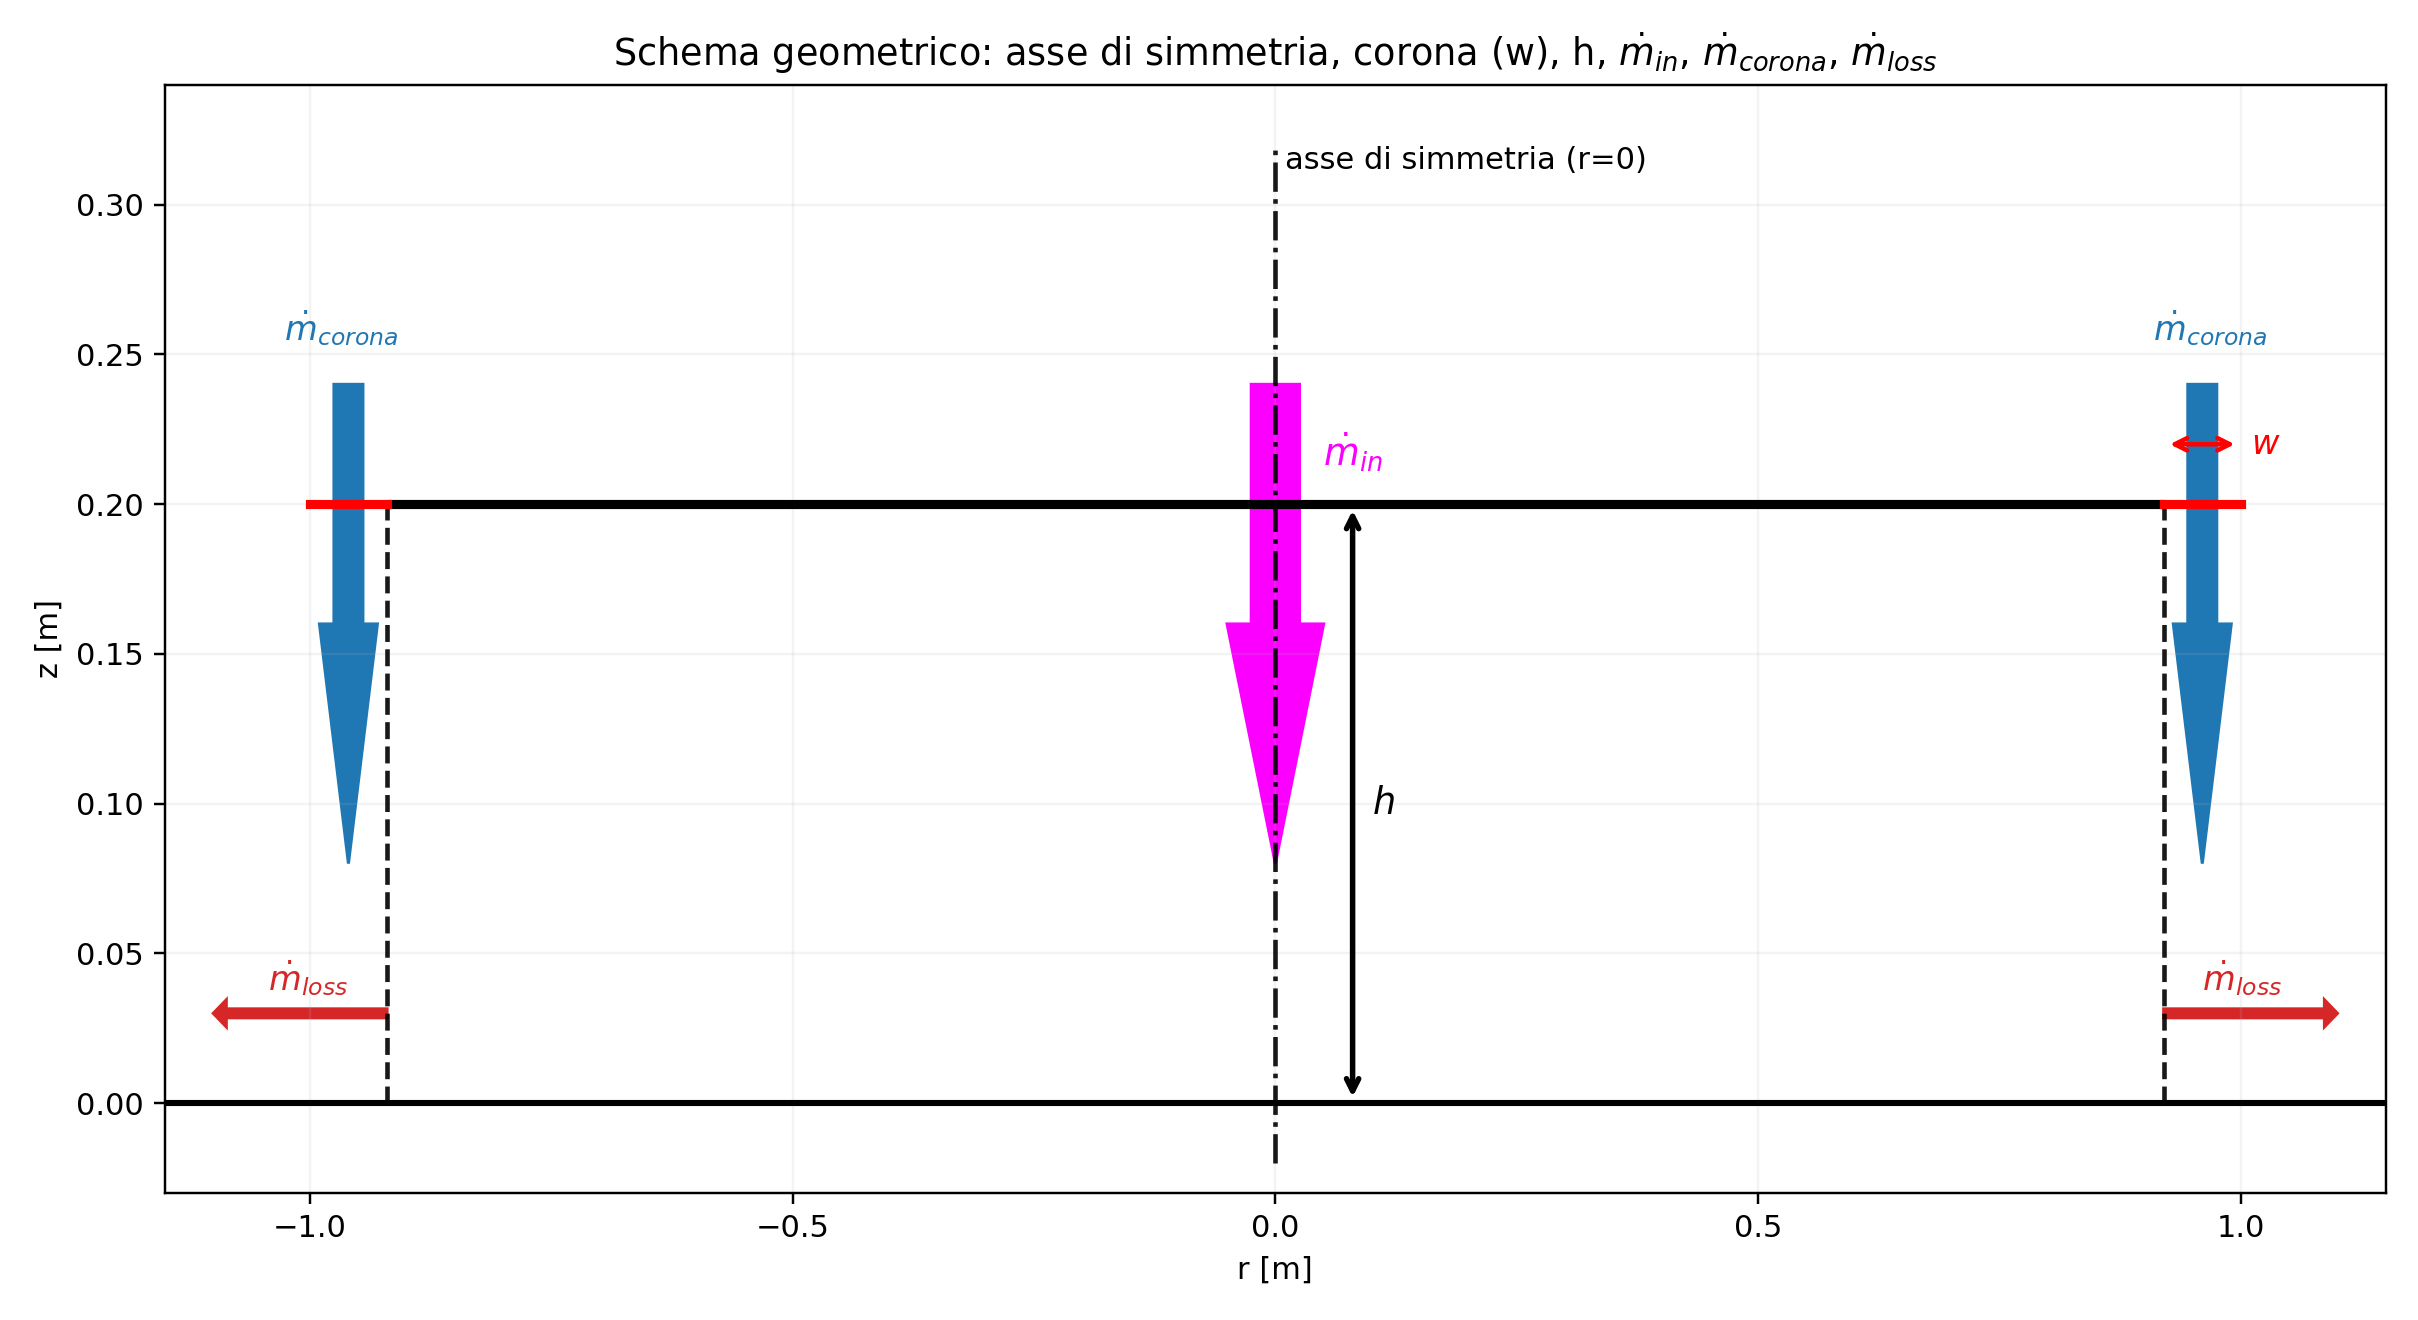
\includegraphics[width=0.95\linewidth]{./figures/schema_geometry.png}
  \caption{Geometric scheme: domain $(r,z)\in[0,R_{\text{tot}}]\times[0,h]$, annulus width $w$, hover height $h$, and the two concentric jets. The outer annular jet forms the air curtain reducing leakage $\dot m_{\mathrm{loss}}$; the inner jet compensates the residual mass loss.}
  \label{fig:geometry}
\end{figure}

\section{Lift Balance}
The hovering condition is set by the pressure force over the planform area ($\pi R_{\text{tot}}^2$):
\begin{equation}
  p_c\,\pi R_{\text{tot}}^2 = W
  \quad \Rightarrow \quad
  p_c = \frac{W}{\pi R_{\text{tot}}^2}.
  \label{eq:lift}
\end{equation}

\section{Leakage Through the Peripheral Gap}
The peripheral annulus governs the mass loss $\dot m_{\mathrm{loss}}$.
Two regimes are considered; the applicable model is selected based on the local Reynolds number
$\mathrm{Re}_h=\rho_\mathrm{edge} U_h h_{\mathrm{eff}}/\mu$, with $U_h\approx Q_{\mathrm{loss}}/(2\pi R_{\text{tot}} h_{\mathrm{eff}})$.

\subsection*{Viscous (lubrication) regime}
\begin{equation}
  Q_{\mathrm{loss}}
  = \frac{\pi h_{\mathrm{eff}}^{3}\,\big(p_\mathrm{edge}-p_0\big)}{6\,\mu\,\ln\!\big(\tfrac{R_{\text{tot}}}{R_{\text{tot}}-w}\big)},
  \qquad \dot m_{\mathrm{loss}}=\rho_\mathrm{edge}\,Q_{\mathrm{loss}}.
  \label{eq:qloss_lub}
\end{equation}

\subsection*{Inertial (orifice) regime}
Let $A_{\mathrm{eff}}=2\pi R_{\text{tot}}\,h_{\mathrm{eff}}$:
\begin{equation}
  Q_{\mathrm{loss}}
  = C_d\,A_{\mathrm{eff}}\,\sqrt{\frac{2\,\big(p_\mathrm{edge}-p_0\big)}{\rho_\mathrm{edge}}},
  \qquad \dot m_{\mathrm{loss}}=\rho_\mathrm{edge}\,Q_{\mathrm{loss}}.
  \label{eq:qloss_orif}
\end{equation}
A smooth interpolation between \eqref{eq:qloss_lub} and \eqref{eq:qloss_orif} can be used in transitional conditions.

\section{Outer Air-Curtain Dynamics (Sealing Condition)}
The outer annular jet, initially vertical at high speed, turns near the ground and acts as a sealing curtain. A momentum balance at the rim yields
\begin{equation}
  p_\mathrm{edge}(z) \;=\; p_0 \;+\;
  C_t\,\frac{\rho_j U_{\mathrm{corona}}^{2}\,b}{h_{\mathrm{eff}}}\,f_z(z),
  \qquad 0\le z\le h,
  \label{eq:curtain_force}
\end{equation}
where $C_t=\mathcal{O}(1)$ collects turning and wall-jet losses, and $f_z(z)$ models the vertical distribution of the curtain pressure loading
(e.g.\ $f_z(z)=1-\lambda z/h$, with $\lambda\in[0.3,0.6]$).

It is convenient to define the nondimensional momentum ratio
\begin{equation}
  J \;\equiv\; \frac{\rho_j U_{\mathrm{corona}}^{2}\,b}{(p_c-p_0)\,h_{\mathrm{eff}}},
  \qquad J\gtrsim J_{\min}=1/C_t,
  \label{eq:J}
\end{equation}
which sets the sealing margin. The corresponding mass flow is
\begin{equation}
  \dot m_{\mathrm{corona}} = \rho_j\,A_{\mathrm{corona}}\,U_{\mathrm{corona}}
  = 2\pi R_{\text{tot}}\,\rho_j\,b\,U_{\mathrm{corona}}.
  \label{eq:mcorona}
\end{equation}
The inward fraction $\beta\in[0,1]$ of the curtain that reinforces the core can be parameterized as
\begin{equation}
  \beta = \frac{1}{1+\gamma\,(h_{\mathrm{eff}}/b)\,J^{-1/2}},\qquad \gamma=\mathcal{O}(1).
  \label{eq:beta}
\end{equation}

\section{Core Model: Compressible, Axisymmetric, Finite Height}
We model the $(r,z)$ core ($0\le r\le R^-, 0\le z\le h$) as a low-Mach compressible flow with no swirl:
\begin{align}
  &\text{\bf Continuity:} &
  \frac{1}{r}\,\partial_r\!\big(r\,\rho u\big)+\partial_z(\rho w)=0,
  \label{eq:cont}\\
  &\text{\bf Momentum (r):} &
  \rho\!\left(u\,\partial_r u+w\,\partial_z u\right)
  = -\partial_r p+\mu\!\left[\partial_r\!\left(\frac{1}{r}\partial_r(ru)\right)+\partial_{zz}u\right],
  \label{eq:momr}\\
  &\text{\bf Momentum (z):} &
  \rho\!\left(u\,\partial_r w+w\,\partial_z w\right)
  = -\partial_z p - \rho g + \mu\!\left[\frac{1}{r}\partial_r\!\left(r\,\partial_r w\right)+\partial_{zz}w\right],
  \label{eq:momz}\\
  &\text{\bf Energy (enthalpy form):} &
  \rho c_p\!\left(u\,\partial_r T+w\,\partial_z T\right)
  = k\!\left[\frac{1}{r}\partial_r\!\left(r\,\partial_r T\right)+\partial_{zz}T\right]+\Phi,
  \label{eq:energy}\\[2pt]
  &\text{\bf State:} &
  p=\rho R_g T.
  \label{eq:state}
\end{align}

For fast design without a full CFD, we adopt an \emph{anisotropic Stokes--Darcy closure} for the mean core velocities:
\begin{equation}
  u = -\frac{\kappa_r}{\mu}\,\partial_r p,\qquad
  w = -\frac{\kappa_z}{\mu}\,\partial_z p,
  \qquad \kappa_r=\alpha_r h^2,\ \kappa_z=\alpha_z h^2,
  \label{eq:darcy}
\end{equation}
with $\alpha_r,\alpha_z$ design parameters (typically $\alpha_r\!\in[0.08,0.2]$, $\alpha_z\!\in[0.02,0.1]$). Combining \eqref{eq:cont} and \eqref{eq:darcy} with $p=\rho R_g T$ yields an \emph{elliptic} equation for $p(r,z)$ that permits vertical pressure variations (driven by $\rho(p,T)$ stratification), consistent with $h\sim R_{\text{tot}}$.

\paragraph{Boundary conditions in the core.}
\begin{itemize}
  \item Axis $r=0$: symmetry, $\partial_r p=0$, $\partial_r T=0$.
  \item Ground $z=0$ and disc underside $z=h$: with the closure \eqref{eq:darcy}, we impose no normal flow ($w=0\Rightarrow \partial_z p=0$); heat exchange via
  $-k\,\partial_n T=h_0\,(T-T_{s0})$ at $z=0$ and $-k\,\partial_n T=h_1\,(T-T_{s1})$ at $z=h$.
  \item Rim $r=R^-$: pressure prescribed by the curtain, $p(R^-,z)=p_\mathrm{edge}(z)$ from \eqref{eq:curtain_force};
  thermal entrainment may be modeled by $-k\,\partial_r T\big|_{R^-}=h_e(z)\,(T(R^-,z)-T_\infty)$.
\end{itemize}

\section{Cushion Mass Balance and Make-Up Flow}
Stationarity requires
\begin{equation}
  \dot m_{\mathrm{in}} + \dot m_{\mathrm{rein}} = \dot m_{\mathrm{loss}}
  \quad\Rightarrow\quad
  \boxed{\ \dot m_{\mathrm{in}} = \dot m_{\mathrm{loss}} - \beta\,\dot m_{\mathrm{corona}}\ }.
  \label{eq:massbalance}
\end{equation}

\section{Power Estimates}
The ideal aerodynamic power is the sum of the cushion power and the jet kinetic power:
\begin{equation}
  P_{\mathrm{ideal}} \approx p_c\,Q_{\mathrm{loss}} + \frac{\dot m_{\mathrm{corona}}\,U_{\mathrm{corona}}^{2}}{2}.
  \label{eq:power}
\end{equation}
With overall efficiency $\eta$ (blower + ducts), $P=P_{\mathrm{ideal}}/\eta$.

\section{Operational Sizing Procedure}
Given $W$ and geometry $R_{\text{tot}},\,h,\,w,\,b$:
\begin{enumerate}
  \item Compute $p_c$ from Eq.~\eqref{eq:lift}.
  \item Choose curtain margin $J$ (or $C_t$), set $U_{\mathrm{corona}}$, $\dot m_{\mathrm{corona}}$ (Eqs.~\eqref{eq:J}--\eqref{eq:mcorona}), and $\beta$ (Eq.~\eqref{eq:beta}).
  \item Set $p_\mathrm{edge}(z)$ from Eq.~\eqref{eq:curtain_force}.
  \item Select leakage regime and compute $Q_{\mathrm{loss}}(p_\mathrm{edge})$ and $\dot m_{\mathrm{loss}}$ (Eqs.~\eqref{eq:qloss_lub}--\eqref{eq:qloss_orif}).
  \item Close the mass balance via Eq.~\eqref{eq:massbalance} to get $\dot m_{\mathrm{in}}$.
  \item Evaluate power with Eq.~\eqref{eq:power}; iterate on $h_{\mathrm{eff}},\,b,\,J,\,w$ to minimize $P$ under stability and safety constraints.
\end{enumerate}

\section{Algorithm for $(r,z)$ Pressure and Velocity Profiles over $0\!-\!h$ and $0\!-\!R_{\text{tot}}$}
We provide a robust low-cost algorithm to compute fields $p(r,z)$ and $\mathbf{v}(r,z)$ on the whole axisymmetric domain without a full CFD:
\begin{enumerate}
  \item \textbf{Inputs:} $R_{\text{tot}},\,w,\,h,\,h_{\mathrm{eff}},\,b,\,W,\,\rho_j,\,U_{\mathrm{corona}},\,T_j,\,T_\infty,\,C_t,\,\lambda,\,C_d,\,\mu,\,k,\,c_p,\,R_g,\,h_0,\,h_1$; closure parameters $\alpha_r,\alpha_z$.
  \item \textbf{Lift \& curtain:} compute $p_c$ (Eq.~\eqref{eq:lift}); set $p_\mathrm{edge}(z)$ via Eq.~\eqref{eq:curtain_force}; get $\dot m_{\mathrm{corona}}$, $\beta$ (Eqs.~\eqref{eq:J}--\eqref{eq:beta}).
  \item \textbf{Leakage:} compute $\dot m_{\mathrm{loss}}$ from Eqs.~\eqref{eq:qloss_lub}--\eqref{eq:qloss_orif} using $\rho_\mathrm{edge}=\rho(p_\mathrm{edge},T_\mathrm{edge})$.
  \item \textbf{Initial temperature field:} solve \eqref{eq:energy} with $u=w=0$ (pure conduction + boundary convection) to obtain $T^{(0)}(r,z)$.
  \item \textbf{Iterative core solve:} for $k=1,2,\dots$:
  \begin{enumerate}
    \item Set $\rho^{(k-1)}=p_c/(R_g T^{(k-1)})$ as initial density field.
    \item Solve the elliptic pressure problem from \eqref{eq:cont}+\eqref{eq:darcy} with $p(R^-,z)=p_\mathrm{edge}(z)$, $\partial_r p(0,z)=0$, $\partial_z p(r,0)=\partial_z p(r,h)=0$, obtaining $p^{(k)}(r,z)$.
    \item Recover velocities from \eqref{eq:darcy}: $u^{(k)}=-(\kappa_r/\mu)\,\partial_r p^{(k)}$, $w^{(k)}=-(\kappa_z/\mu)\,\partial_z p^{(k)}$.
    \item Enforce global mass balance: compute the outflow $\dot m_{\mathrm{loss}}^{(k)}=\int_0^h \rho(p^{(k)},T^{(k-1)})\,u^{(k)}(R^-,z)\,dz$; if $\dot m_{\mathrm{loss}}^{(k)}$ differs from step 3, adjust $\alpha_r,\alpha_z$ or $p_\mathrm{edge}$ (via $U_{\mathrm{corona}}$) and repeat.
    \item Solve energy \eqref{eq:energy} with advection by $(u^{(k)},w^{(k)})$ and boundary heat transfer to get $T^{(k)}(r,z)$.
    \item Convergence: stop when $\norm{p^{(k)}-p^{(k-1)}}_\infty/p_c<10^{-2}$ and $\norm{T^{(k)}-T^{(k-1)}}_\infty/T_\infty<10^{-2}$.
  \end{enumerate}
  \item \textbf{Outputs:} maps $p(r,z)$, $T(r,z)$, $u(r,z)$, $w(r,z)$; derived quantities: $\dot m_{\mathrm{loss}}$, $\dot m_{\mathrm{in}}$, shear at $z=0$ and $z=h$, and power.
\end{enumerate}

\section{Calibration and Design Parameters}
Lumped parameters to be validated experimentally on the target geometry: (i) $C_t$ and $f_z(z)$ for the curtain loading, (ii) the inward fraction $\beta$ (or its parameter $\gamma$), (iii) the discharge coefficient $C_d$ for inertial leakage, and (iv) the anisotropic permeabilities $\kappa_r=\alpha_r h^2$, $\kappa_z=\alpha_z h^2$ used in the Stokes--Darcy closure.

\end{document}
